\documentclass[10pt]{beamer}
\usetheme{Warsaw}
\usecolortheme{beaver}

\usepackage{amssymb, amsmath, amsfonts}
\usepackage{moreverb}
\usepackage{graphicx}
\usepackage{enumerate}
\usepackage{graphics}
\usepackage{color}
\usepackage{array}
\usepackage{float}
\usepackage{hyperref}
\usepackage{textcomp}
\usepackage{alltt}
\usepackage{mathtools}
\usepackage{tikz}
\usetikzlibrary{positioning}
\usetikzlibrary{arrows}
\usepackage{pgfplots}
\usepackage{bigints}

\newcommand{\suchthat}{\, \mid \,}
\renewcommand{\theenumi}{\alph{enumi}}
\newcommand\Wider[2][3em]{%
\makebox[\linewidth][c]{%
  \begin{minipage}{\dimexpr\textwidth+#1\relax}
  \raggedright#2
  \end{minipage}%
  }%
}

\pgfmathdeclarefunction{gauss}{2}{%
  \pgfmathparse{1/(#2*sqrt(2*pi))*exp(-((x-#1)^2)/(2*#2^2))}%
}

\setcounter{section}{-1}
%\setlength{\jot}{30pt}

\title{The Ecological Effects of Trait Variation in a $u$-Predator, $v$-Prey System}
\author{Sam Fleischer, Pablo Chavarria}
\date{May 3, 2015}

\begin{document}

\begin{frame}
	\titlepage
	\begin{center}
		{\bf Preparing Undergraduates through Mentoring for PhDs (PUMP) Research Symposium}
	\end{center}
	\begin{align*}
		\begin{array}{lll}
		\text{Advisor:} & \text{Dr. Jing Li, Mathematics,} & \text{CSU Northridge} \\
		\text{Consultant:} & \text{Dr. Casey terHorst, Biology,} & \text{CSU Northridge} \\
		\text{Supported By:} & \text{Pacific Math Alliance, PUMP,} & \text{CSU Northridge}
		\end{array}
	\end{align*}
\end{frame}

\begin{frame}
	\frametitle{Overview}
	\begin{itemize}
		\item Motivation / Observations in Nature
		\item Model Formulation
		\begin{itemize}
			\item Classical Lotka-Volterra Predator-Prey Model
			\item Schreiber, B\"urger, and Bolnick's Extension
			\item Our Extension
		\end{itemize}
		\item Preliminary Results
		\item Future Work
	\end{itemize}
\end{frame}

\section{Motivation / Observations in Nature}
\begin{frame}
	\frametitle{Motivation / Observations in Nature}
\begin{minipage}{0.65\textwidth}
	\begin{itemize}
		\item Predator/Prey interactions are prevalent in nature
		\begin{itemize}
			\item Crab vs. gastropod {\tiny[Saloniemi, 1993]}
			\item Protist vs. bacteria {\tiny[terHorst]}
		\end{itemize}
		\item There is trait variation within species
		\begin{itemize}
			\item Thickness of plant cuticula {\tiny[Saloniemi, 1993]}
			\item Strength of gastropod shell {\tiny[Saloniemi, 1993]}
		\end{itemize}
		\item Incorporating trait variation provides {\bf richer dynamics} than classical Lotka-Volterra models
	\end{itemize}
	\end{minipage}
	\begin{minipage}{0.25\textwidth}
	\begin{figure}
	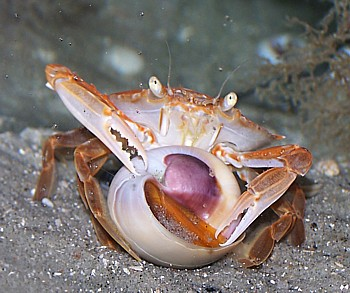
\includegraphics[width=0.95\textwidth]{figures/crab_eating_gastropod.jpg}
	\end{figure}
	\end{minipage}
\end{frame}

\section{Model Formulation}
\subsection{Lotka-Volterra}
\begin{frame}
	\frametitle{Classical Lotka-Volterra Model}
	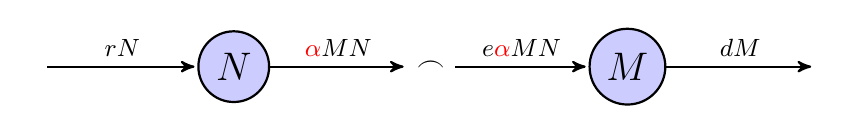
\begin{tikzpicture}[->,>=stealth',shorten >=1pt,auto,node distance=2.5cm, thick,main node/.style={circle,fill=blue!20,draw,font=\sffamily\Large\bfseries}]

		\node[main node] (1) {$N$};
		\node (midpt) [right of=1] {$\frown$};
		\node[main node] (2) [right of=midpt] {$M$};
		\node (input) [left of=1] {};
		\node (output) [right of=2] {};

		\path[every node/.style={font=\sffamily\small}]
		(input)	edge node {$rN$} (1)
		(1)		edge node {${\color{red}\alpha} MN$} (midpt)
		(midpt)	edge node {$e{\color{red}\alpha} MN$} (2)
		(2)		edge node {$dM$} (output);
	\end{tikzpicture}\vskip0.75cm
	\begin{columns}
    		\begin{column}{0.35\textwidth}
			\begin{align*}
				\frac{dN}{dt} &= N(r - {\color{red}\alpha} M)\\[.1cm]
				\frac{dM}{dt} &= M(e{\color{red}\alpha} N - d)
			\end{align*}
   		 \end{column}
		 \begin{column}{0.60\textwidth}
			{\bf Variables}
			\begin{itemize}
				\item $N \equiv $ Prey Density
				\item $M \equiv $ Predator Density
			\end{itemize}
			{\bf Parameters}
			\begin{itemize}
				\item {\color{red}$\alpha \equiv $ Attack rate\uncover<2->{\ \ \ \ \ $\longleftarrow$ {\bf No variation!}}}
				\item $r \equiv $ Prey birth rate
				\item $e \equiv $ Efficiency
				\item $d \equiv $ Predator death rate
			\end{itemize}
		\end{column}
	\end{columns}
\end{frame}
\subsection{Schreiber, B\"urger, and Bolnick}
\begin{frame}
	\frametitle{Schreiber, B\"urger, and Bolnick's Extension}
	{\bf Assume the {\color{red}Predator Species} has a normally distributed trait value.}
	\begin{align*}
		p({\color{red}m}, \overline{m}) &= \frac{1}{\sqrt{2\pi\sigma^2}}\exp\left[{-\frac{({\color{red}m} - \overline{m})^2}{2\sigma^2}}\right]
	\end{align*}
	\uncover<2->{{\bf Attack Rate is a Function of the {\color{red}Predator's Trait Value}}
	\begin{align*}
		a({\color{red}m}) &= \alpha \exp\left[-\frac{({\color{red}m} - {\color{cyan}\theta})^2}{2\tau^2}\right]
	\end{align*}}
	\begin{columns}
		\begin{column}{0.45\textwidth}
			{\bf Variables}
			\begin{itemize}
				\item {\color{red}$m \equiv $ Predator Trait Value}
				\item \uncover<3->{{\color{blue} (((No Prey Trait Value)))}}
			\end{itemize}
		\end{column}
		\begin{column}{0.60\textwidth}
			{\bf Parameters}
			\begin{itemize}
				\item $\sigma^2 \equiv $ Predator Trait Variance
				\item \uncover<2->{$\alpha \equiv $ Maximum attack rate}
				\item \uncover<2->{$\tau \equiv $ Specialization Constant}
				\item \uncover<2->{{\color{cyan}$\theta \equiv $ Optimal trait value \uncover<3->{\\ \ \ \ \ \ \ $\uparrow$ {\bf No variation!}}}}
			\end{itemize}
		\end{column}
	\end{columns}
\end{frame}
\subsection*{Our Extension}
\begin{frame}
	\frametitle{Normally Distributed Trait Values}
	{\bf Assume {\color{blue}Prey} and {\color{red}Predator} have normally distributed trait values.}
	\begin{align*}
		p({\color{blue}n}, {\color{blue}\overline{n}}) &= \frac{1}{\sqrt{2\pi\beta^2}}\exp\left[{-\frac{({\color{blue}n} - {\color{blue}\overline{n}})^2}{2\beta^2}}\right]
	\end{align*}
	\begin{align*}
		p({\color{red}m}, {\color{red}\overline{m}}) &= \frac{1}{\sqrt{2\pi\sigma^2}}\exp\left[{-\frac{({\color{red}m} - {\color{red}\overline{m}})^2}{2\sigma^2}}\right]
	\end{align*}
	\begin{columns}
		\begin{column}{0.50\textwidth}
			{\bf Variables}
			\begin{itemize}
				\item \footnotesize{\color{blue}$n \equiv $ Prey Trait Value}
				\item {\color{blue}$\overline{n} \equiv $ {\bf Average} Prey Trait Value}
				\item {\color{red}$m \equiv $ Predator Trait Value}
				\item {\color{red}$\overline{m} \equiv $ {\bf Average} Predator Trait Value}
			\end{itemize}
		\end{column}
		\begin{column}{0.42\textwidth}
			{\bf Parameters}
			\begin{itemize}
				\item \footnotesize$\beta^2 \equiv $ Prey Trait Variance
				\item $\sigma^2 \equiv $ Predator Trait Variance
			\end{itemize}
		\end{column}
	\end{columns}

\end{frame}
\begin{frame}
	\frametitle{{\large Attack Rate as a function of Normally Distributed Trait Values}}
	{\bf Attack Rate is a Function of the {\color{blue}Prey's Trait Value} and the {\color{red}Predator's Trait Value}}
	\begin{align*}
		a({\color{blue}n}, {\color{red}m}) &= \alpha \exp\left[-\frac{(({\color{red}m} - {\color{blue}n}) - {\color{cyan}\theta})^2}{2\tau^2}\right]
	\end{align*}
	\uncover<2->{{\bf Average Attack Rate}
	\begin{align*}
		\overline{a}({\color{blue}\overline{n}}, {\color{red}\overline{m}}) &= \int_{-\infty}^{\infty}\int_{\-\infty}^{\infty} a({\color{blue}n}, {\color{red}m}) \cdot p({\color{blue}n}, {\color{blue}\overline{n}}) \cdot p({\color{red}m}, {\color{red}\overline{m}})\ d{\color{blue}n} d{\color{red}m} \\
		&= \frac{\alpha\tau}{\sqrt{\sigma^2 + \beta^2 + \tau^2}}\exp\left[{-\frac{(({\color{red}\overline{m}} - {\color{blue}\overline{n}}) - {\color{cyan}\theta})^2}{2(\sigma^2 + \beta^2 + \tau^2)}}\right]
	\end{align*}}
	\begin{columns}
		\begin{column}{0.50\textwidth}
			{\bf Variables}
			\begin{itemize}
				\item \footnotesize{\color{blue}$n \equiv $ Prey Trait Value}
				\item {\color{blue}$\overline{n} \equiv $ {\bf Average} Prey Trait Value}
				\item {\color{red}$m \equiv $ Predator Trait Value}
				\item {\color{red}$\overline{m} \equiv $ {\bf Average} Predator Trait Value}
			\end{itemize}
		\end{column}
		\begin{column}{0.42\textwidth}
			{\bf Parameters}
			\begin{itemize}
				\item \footnotesize$\alpha \equiv $ Maximum attack rate
				\item {\color{cyan}$\theta \equiv $ Optimal trait \bf difference}
				\item $\tau^2 \equiv $ Specialization Constant
				\item \uncover<2->{$\beta^2 \equiv $ Prey Trait Variance}
				\item \uncover<2->{$\sigma^2 \equiv $ Predator Trait Variance}
			\end{itemize}
		\end{column}
	\end{columns}
\end{frame}
\begin{frame}
	\frametitle{Fitness Assumptions}
	\begin{itemize}
		\item Prey experiences {\color{blue}logistic growth} in absence of predator
		\item Predator experiences {\color{red}exponential decay} in absence of prey
	\end{itemize}
	\begin{align*}
		Y(N, n, M, m) &= {\color{blue}r\left(1 - \frac{N}{K}\right)} - Ma(n, m) \\[.1cm]
		W(N, n, M, m) &= eNa(n, m)\ {\color{red}-\ d}
	\end{align*}
	\begin{columns}
		\begin{column}{0.45\textwidth}
			{\bf Variables}
			\begin{itemize}
				\item \footnotesize$N \equiv $ Prey Density
				\item $n \equiv $ Prey Trait Value
				\item $M \equiv $ Predator Density
				\item $m \equiv $ Predator Trait Value
			\end{itemize}
		\end{column}
		\begin{column}{0.55\textwidth}
			{\bf Parameters}
			\begin{itemize}
				\item \footnotesize{\color{blue}$r \equiv $ Intrinsic Prey Growth Rate}
				\item {\color{blue}$K \equiv $ Prey Carrying Capacity}
				\item {\color{red}$d \equiv $ Predator Death Rate}
				\item $e \equiv $ Efficiency
			\end{itemize}
		\end{column}
	\end{columns}
\end{frame}
\begin{frame}
	\frametitle{Average Fitness}
	\begin{align*}
	{\color{blue}\overline{Y}(N, \overline{n}, M, \overline{m})} &= \int_{-\infty}^{\infty}\int_{-\infty}^{\infty} Y(N, n, M, m) \cdot p(m, \overline{m}) \cdot p(n, \overline{n})\ dm dn \\
	&= {\color{blue}r\left(1 - \frac{N}{K}\right) - M\overline{a}(\overline{n}, \overline{m})} \\[.1cm]
	{\color{red}\overline{W}(N, \overline{n}, M, \overline{m})} &= \int_{-\infty}^{\infty}\int_{-\infty}^{\infty} W(N, n, M, m) \cdot p(m, \overline{m}) \cdot p(n, \overline{n})\ dm dn \\
	&= {\color{red}eN\overline{a}(\overline{n}, \overline{m}) - d}
	\end{align*}
	\begin{columns}
		\begin{column}{0.45\textwidth}
			{\bf Variables}
			\begin{itemize}
				\item \footnotesize{\color{blue}$N \equiv $ Prey Density}
				\item {\color{blue}$\overline{n} \equiv $ {\bf Average} Prey Trait Value}
				\item {\color{red}$M \equiv $ Predator Density}
				\item {\color{red}$\overline{m} \equiv $ {\bf Average} Predator Trait \hphantom{$\overline{m} \equiv $} Value}
			\end{itemize}
		\end{column}
		\begin{column}{0.55\textwidth}
			{\bf Parameters}
			\begin{itemize}
				\item \footnotesize$\overline{r} \equiv $ Intrinsic Prey Growth Rate
				\item $K \equiv $ Prey Carrying Capacity
				\item $d \equiv $ Predator Death Rate
				\item $e \equiv $ Efficiency
			\end{itemize}
		\end{column}
	\end{columns}
\end{frame}
\begin{frame}
	\frametitle{Ecological Components}
	\begin{align*}
		\frac{dN}{dt} &= N\cdot {\color{blue}\overline{Y}(N, \overline{n}, M, \overline{m})}\ = N{\color{blue}\left[r\left(1 - \frac{N}{K}\right) - M\overline{a}(\overline{n}, \overline{m})\right]}\\[.1cm]
		\frac{dM}{dt} &= M\cdot {\color{red}\overline{W}(N, \overline{n}, M, \overline{m})} = M{\color{red}\left[eN\overline{a}(\overline{n}, \overline{m}) - d\right]}
	\end{align*}\vskip0.15cm
	\begin{center}
		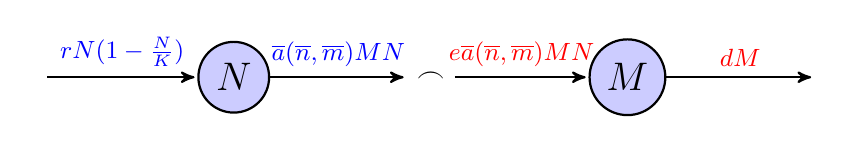
\begin{tikzpicture}[->,>=stealth',shorten >=1pt,auto,node distance=2.5cm, thick,main node/.style={circle,fill=blue!20,draw,font=\sffamily\Large\bfseries}]
	
			\node[main node] (1) {$N$};
			\node (midpt) [right of=1] {$\frown$};
			\node[main node] (2) [right of=midpt] {$M$};
			\node (input) [left of=1] {};
			\node (output) [right of=2] {};
	
			\path[every node/.style={font=\sffamily\small}]
			(input)	edge node {{\color{blue}$rN(1 - \frac{N}{K})$}} (1)
			(1)		edge node {{\color{blue}$\overline{a}(\overline{n}, \overline{m})MN$}} (midpt)
			(midpt)	edge node {{\color{red}$e\overline{a}(\overline{n}, \overline{m})MN$}} (2)
			(2)		edge node {{\color{red}$dM$}} (output);
		\end{tikzpicture}\vskip0.35cm
	\end{center}
	\vskip.25cm
	\begin{columns}
		\begin{column}{0.5\textwidth}
			{\bf Variables}
			\begin{itemize}
				\item \footnotesize{\color{blue}$N \equiv $ Prey Density}
				\item {\color{blue}$\overline{n} \equiv $ {\bf Average} Prey Trait Value}
				\item {\color{red}$M \equiv $ Predator Density}
				\item {\color{red}$\overline{m} \equiv $ {\bf Average} Predator Trait Value}
			\end{itemize}
		\end{column}
		\begin{column}{0.5\textwidth}
			{\bf Parameters}
			\begin{itemize}
				\item \footnotesize$\overline{r} \equiv $ Intrinsic Prey Growth Rate
				\item $K \equiv $ Prey Carrying Capacity
				\item $d \equiv $ Predator Death Rate
				\item $e \equiv $ Efficiency
			\end{itemize}
		\end{column}
	\end{columns}
\end{frame}
\begin{frame}
	\frametitle{Evolutionary Components}
	\begin{itemize}
		\item The evolution of the mean trait value is always \underline{in the direction} \underline{which increases the mean fitness in the population}. {\tiny[Lande, 1976]}
	\end{itemize}
	\begin{align*}
	\frac{d\overline{n}}{dt} &= \beta_G^2{\color{cyan}\frac{\partial \overline{Y}}{\partial \overline{n}}} = \beta_G^2{\color{cyan}\frac{M(\theta - (\overline{m} - \overline{n}))}{\sigma^2 + \beta^2 + \tau^2} \overline{a}(\overline{m}, \overline{n})}\\[.1cm]
	\frac{d\overline{m}}{dt} &= \sigma_G^2{\color{magenta}\frac{\partial \overline{W}}{\partial \overline{m}}} = \sigma_G^2{\color{magenta}\frac{eN(\theta - (\overline{m} - \overline{n}))}{\sigma^2 + \beta^2 + \tau^2} \overline{a}(\overline{m}, \overline{n})}
	\end{align*}
	\vskip.25cm
	\begin{columns}
		\begin{column}{0.5\textwidth}
			{\bf Variables}
			\begin{itemize}
				\item $N \equiv $ Prey Density
				\item $\overline{n} \equiv $ Mean Prey Character
				\item $M \equiv $ Predator Density
				\item $\overline{m} \equiv $ Mean Predator Character
			\end{itemize}
		\end{column}
		\begin{column}{0.5\textwidth}
			{\bf Parameters}
			\begin{itemize}
				\item $\beta_G^2 \equiv $ Prey genetic variance
				\item $\sigma_G^2 \equiv $ Predator genetic variance
			\end{itemize}
		\end{column}
	\end{columns}
\end{frame}
\begin{frame}
	\frametitle{The Complete $1\times1$ Model \\ (One Predator Species, One Prey Species)}
	{\bf Ecological Components}
	\begin{align*}
	\frac{dN}{dt} &= N\cdot {\color{blue}\overline{Y}(\overline{m}, \overline{n}, M, N)}\ \ =\ N{\color{blue}\left[r\left(1 - \frac{N}{K}\right) - M\overline{a}(\overline{m}, \overline{n})\right]}\\[.1cm]
	\frac{dM}{dt} &= M\cdot {\color{red}\overline{W}(\overline{m}, \overline{n}, N)}\ \ \ \ \ =\ M{\color{red}\left[eN\overline{a}(\overline{m}, \overline{n}) - d\right]}
	\end{align*}
	{\bf Evolutionary Components}
	\begin{align*}
	\frac{d\overline{n}}{dt} &= \beta_G^2{\color{cyan}\frac{\partial \overline{Y}}{\partial \overline{n}}} = \beta_G^2{\color{cyan}\frac{M(\theta + \overline{n} - \overline{m})}{\sigma^2 + \beta^2 + \tau^2} \overline{a}(\overline{m}, \overline{n})}\\[.1cm]
	\frac{d\overline{m}}{dt} &= \sigma_G^2{\color{magenta}\frac{\partial \overline{W}}{\partial \overline{m}}} = \sigma_G^2{\color{magenta}\frac{eN(\theta + \overline{n} - \overline{m})}{\sigma^2 + \beta^2 + \tau^2} \overline{a}(\overline{m}, \overline{n})}
	\end{align*}
\end{frame}

\begin{frame}
	\frametitle{Equilibria - $1\times1$}
	\begin{align*}
		\begin{array}{ll}
			\dfrac{dN}{dt} = N\cdot {\color{blue}\overline{Y}(\overline{m}, \overline{n}, M, N)} &\ \ \ \ \ \ \dfrac{d\overline{n}}{dt} = \beta_G^2{\color{cyan}\dfrac{\partial \overline{Y}}{\partial \overline{n}}} \\[.3cm]
			\dfrac{dM}{dt} = M\cdot {\color{red}\overline{W}(\overline{m}, \overline{n}, N)} & \ \ \ \ \ \ \dfrac{d\overline{m}}{dt} = \sigma_G^2{\color{magenta}\dfrac{\partial \overline{W}}{\partial \overline{m}}}
		\end{array}
	\end{align*}
	{\bf Extinction} \uncover<2->{$\boxed{\text{\it Unstable}}$}
	\begin{align*}
		(N^*, M^*, \overline{n}^*, \overline{m}^*) = (0, 0, \underline{\ \ }, \underline{\ \ })
	\end{align*}
	{\bf Exclusion} \uncover<3->{$\boxed{\text{\it Stable under certain conditions}}$}
	\begin{align*}
		(N^*, M^*, \overline{n}^*, \overline{m}^*) = (K, 0, \underline{\ \ }, \underline{\ \ })
	\end{align*}
	\uncover<4->{{\bf Necessary Conditions for Stable Exclusion:}}
	\begin{itemize}
		\item \uncover<4->{$d > e\overline{a}(\overline{m}^*, \overline{n}^*)K$}
		\item \uncover<4->{$(\overline{m}^* - \overline{n}^* - \theta)^2 < \sigma^2 + \beta^2 + \tau^2$}
	\end{itemize}
\end{frame}
\begin{frame}
	\frametitle{Equilibria - $1\times1$}
	\begin{align*}
		\begin{array}{ll}
			\dfrac{dN}{dt} = N\cdot {\color{blue}\overline{Y}(\overline{m}, \overline{n}, M, N)} &\ \ \ \ \ \ \dfrac{d\overline{n}}{dt} = \beta_G^2{\color{cyan}\dfrac{\partial \overline{Y}}{\partial \overline{n}}} \\[.3cm]
			\dfrac{dM}{dt} = M\cdot {\color{red}\overline{W}(\overline{m}, \overline{n}, N)} & \ \ \ \ \ \ \dfrac{d\overline{m}}{dt} = \sigma_G^2{\color{magenta}\dfrac{\partial \overline{W}}{\partial \overline{m}}}
		\end{array}
	\end{align*}
	{\bf Coexistence} \uncover<2->{$\boxed{\text{\it Stable under certain conditions}}$}
	\begin{align*}
		(N^*, M^*, \overline{n}^*, \overline{m}^*) = (\dfrac{d\sqrt{A}}{e \alpha \tau}\ ,\ \dfrac{r\sqrt{A}}{\alpha\tau}\left(1 - \dfrac{d\sqrt{A}}{Ke\alpha\tau}\right)\ ,\ \mu^*\ ,\ \mu^* - \theta) \\[.1cm]
		\text{where $A = \sigma^2 + \beta^2 + \tau^2$ and $\mu^*$ is an arbitrary value.}
	\end{align*}
	\uncover<3->{{\bf Necessary Condition for Stable Coexistence:}}
	\begin{itemize}
		\item \uncover<3->{$d\sigma_G^2 > r\beta_G^2\left(1 - \dfrac{d\sqrt{A}}{Ke\alpha\tau}\right)$}
	\end{itemize}
\end{frame}

\begin{frame}
	\frametitle{Figures - $1\times1$ - Stable Exclusion}
	\Wider[6em]{
	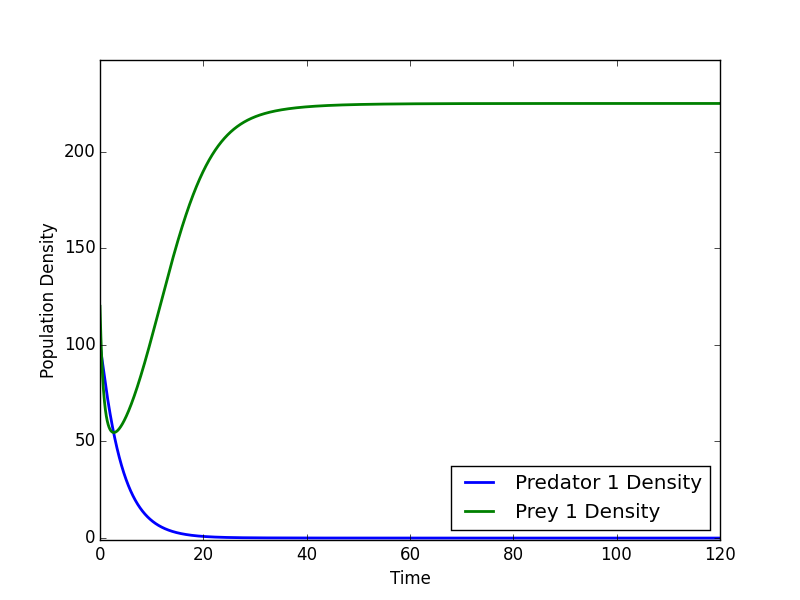
\includegraphics[scale=0.3175]{figures/1x1/constant_growth/densities_exclusion.png}
   	\hfill
   	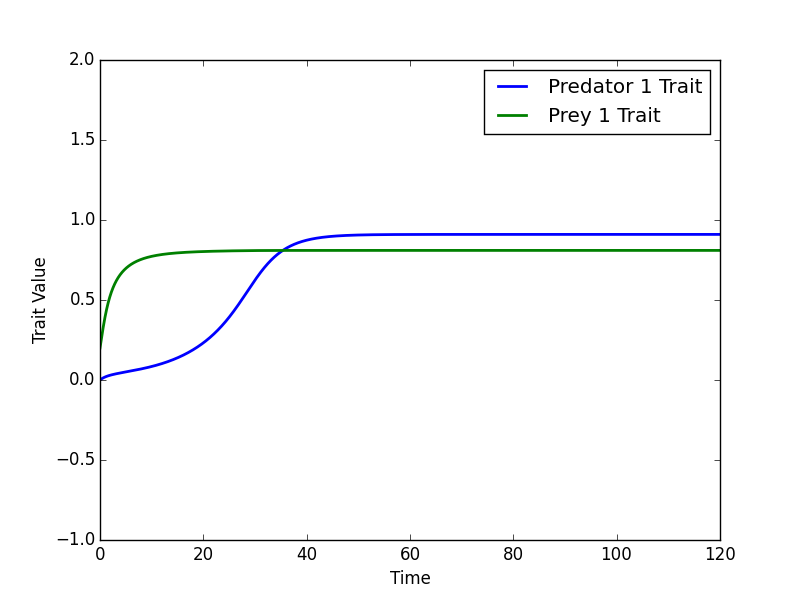
\includegraphics[scale=0.3175]{figures/1x1/constant_growth/traits_exclusion.png}
	}
\end{frame}
\begin{frame}
	\frametitle{Figures - $1\times1$ - Stable Coexistence}
	\Wider[6em]{
	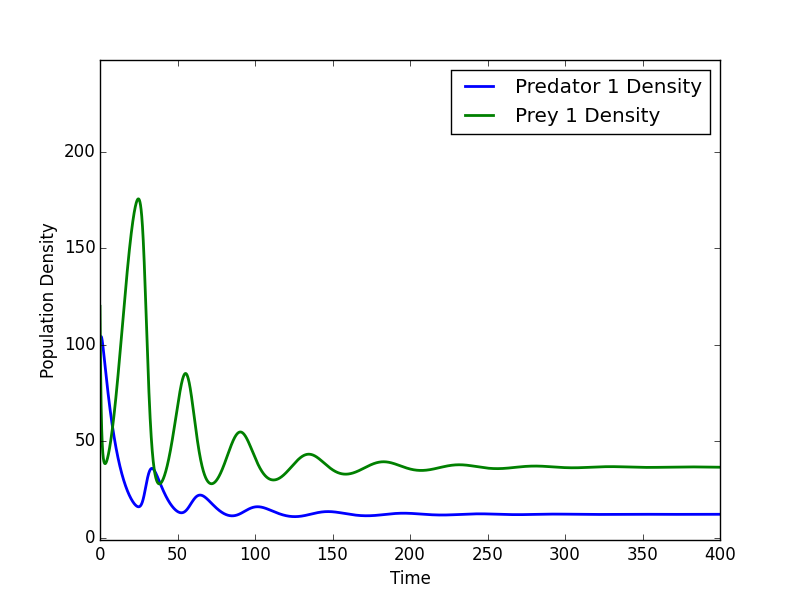
\includegraphics[scale=0.3175]{figures/1x1/constant_growth/densities_stable_coexistence.png}
   	\hfill
   	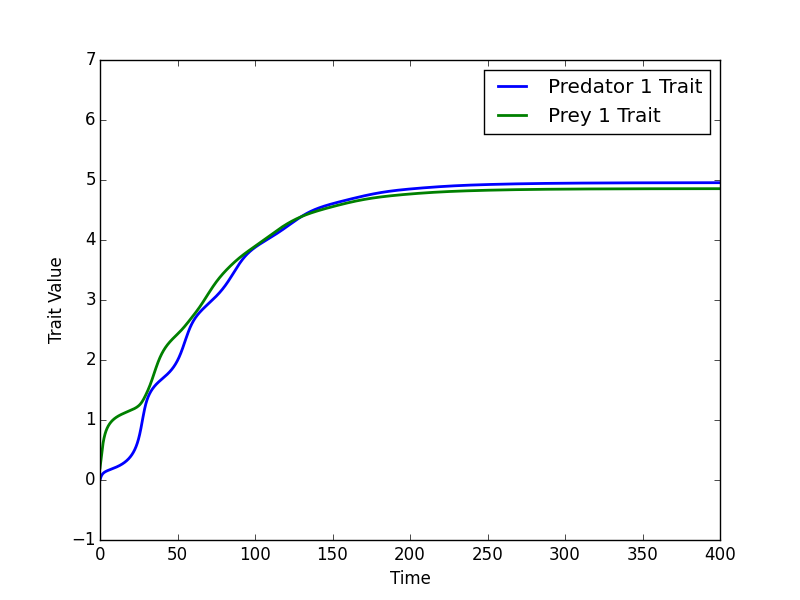
\includegraphics[scale=0.3175]{figures/1x1/constant_growth/traits_stable_coexistence.png}
	}
\end{frame}
\begin{frame}
	\frametitle{Figures - $1\times1$ - ``Arms Race'' Coexistence}
	\Wider[6em]{
	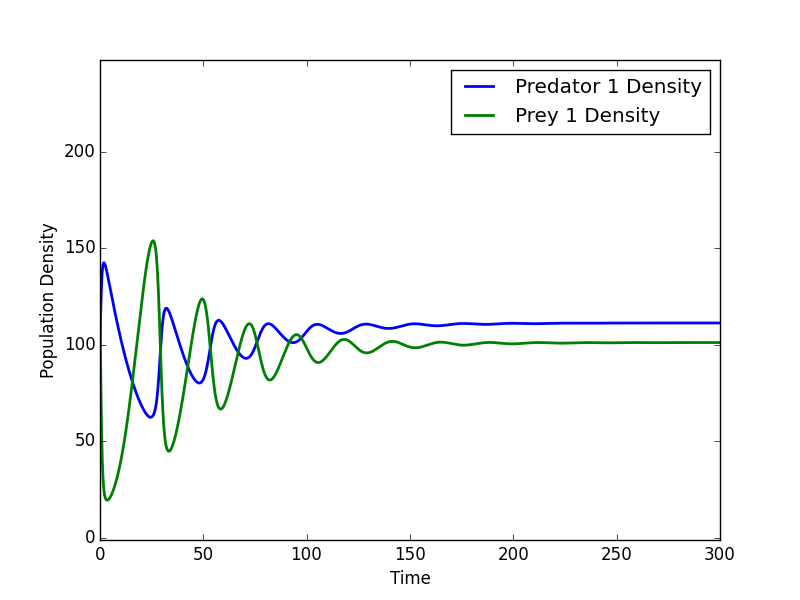
\includegraphics[scale=0.3175]{figures/1x1/constant_growth/densities_unstable_coexistence.png}
   	\hfill
   	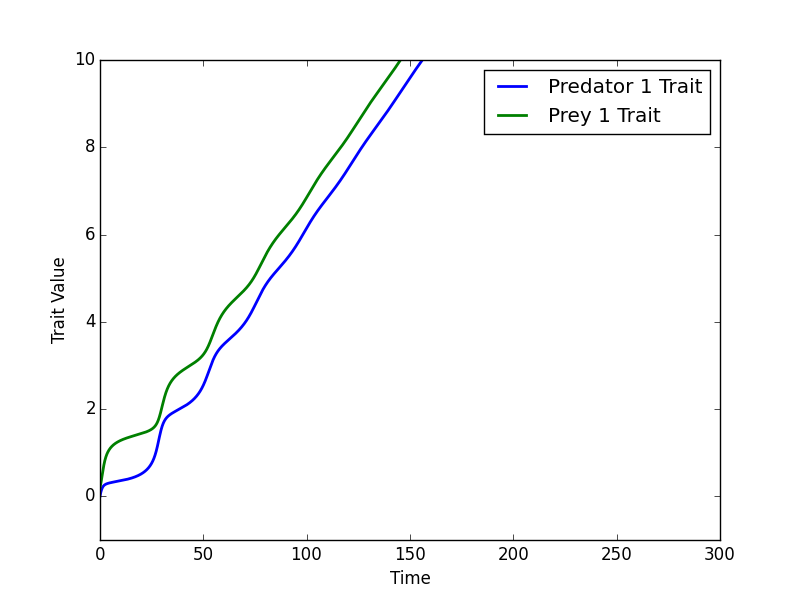
\includegraphics[scale=0.3175]{figures/1x1/constant_growth/traits_unstable_coexistence.png}
	}
\end{frame}
\begin{frame}
	\frametitle{Avoiding an ``Arms Race'' with Stabilizing Selection}
	{\bf Assume Prey Growth Rate is a Function of the {\color{blue}Prey's Trait Value}}
	\begin{align*}
		r({\color{blue}n}) &= \rho \exp\left[-\frac{({\color{blue}n} - \phi)^2}{2\gamma^2}\right]
	\end{align*}
	\uncover<2->{{\bf Averge Growth Rate}}
	\uncover<2->{\begin{align*}
		\overline{r}({\color{blue}\overline{n}}) &= \int_{-\infty}^{\infty}r({\color{blue}n}) \cdot p({\color{blue}n}, {\color{blue}\overline{n}}) d{\color{blue}n} \\
		&= \frac{\rho\gamma}{\sqrt{\beta^2 + \gamma^2}}\exp{\left[-\frac{({\color{blue}n} - \phi)^2}{2\gamma^2}\right]}
	\end{align*}}
	\begin{columns}
		\begin{column}{0.42\textwidth}
			{\bf Variables}
			\begin{itemize}
				\item \footnotesize{\color{blue}$n \equiv $ Prey Trait Value}
				\item {\color{blue}$\overline{n} \equiv $ {\bf Average} Prey Trait Value}
			\end{itemize}
		\end{column}
		\begin{column}{0.48\textwidth}
			{\bf Parameters}
			\begin{itemize}
				\item \footnotesize$\rho \equiv $ Maximum Growth Rate
				\item $\phi \equiv $ Prey Optimum Trait Value
				\item $\gamma^2 \equiv $ Stabilizing Selection Constant
				\item \uncover<2->{$\beta^2 \equiv $ Prey Trait Variance}
			\end{itemize}
		\end{column}
	\end{columns}
\end{frame}
\begin{frame}
	\frametitle{Fitness Assumptions}
	\begin{itemize}
		\item Prey experiences {\color{blue}logistic growth} in absence of predator
		\item Predator experiences {\color{red}exponential decay} in absence of prey
	\end{itemize}
	\begin{align*}
		Y(N, n, M, m) &= {\color{blue}r(n)\left(1 - \frac{N}{K}\right)} - Ma(n, m) \\[.1cm]
		W(N, n, M, m) &= eNa(n, m)\ {\color{red}-\ d}
	\end{align*}
	\begin{columns}
		\begin{column}{0.45\textwidth}
			{\bf Variables}
			\begin{itemize}
				\item \footnotesize$N \equiv $ Prey Density
				\item $n \equiv $ Prey Trait Value
				\item $M \equiv $ Predator Density
				\item $m \equiv $ Predator Trait Value
			\end{itemize}
		\end{column}
		\begin{column}{0.55\textwidth}
			{\bf Parameters}
			\begin{itemize}
				\item \footnotesize{\color{blue}$r \equiv $ Intrinsic Prey Growth Rate Function}
				\item {\color{blue}$K \equiv $ Prey Carrying Capacity}
				\item {\color{red}$d \equiv $ Predator Death Rate}
				\item $e \equiv $ Efficiency
			\end{itemize}
		\end{column}
	\end{columns}
\end{frame}
\begin{frame}
	\frametitle{Average Fitness}
	\begin{align*}
	{\color{blue}\overline{Y}(N, \overline{n}, M, \overline{m})} &= \int_{-\infty}^{\infty}\int_{-\infty}^{\infty} Y(N, n, M, m) \cdot p(m, \overline{m}) \cdot p(n, \overline{n})\ dm dn \\
	&= {\color{blue}\overline{r}(\overline{n})\left(1 - \frac{N}{K}\right) - M\overline{a}(\overline{n}, \overline{m})} \\[.1cm]
	{\color{red}\overline{W}(N, \overline{n}, M, \overline{m})} &= \int_{-\infty}^{\infty}\int_{-\infty}^{\infty} W(N, n, M, m) \cdot p(m, \overline{m}) \cdot p(n, \overline{n})\ dm dn \\
	&= {\color{red}eN\overline{a}(\overline{n}, \overline{m}) - d}
	\end{align*}
	\begin{columns}
		\begin{column}{0.45\textwidth}
			{\bf Variables}
			\begin{itemize}
				\item \footnotesize{\color{blue}$N \equiv $ Prey Density}
				\item {\color{blue}$\overline{n} \equiv $ {\bf Average} Prey Trait Value}
				\item {\color{red}$M \equiv $ Predator Density}
				\item {\color{red}$\overline{m} \equiv $ {\bf Average} Predator Trait \hphantom{$\overline{m} \equiv $} Value}
			\end{itemize}
		\end{column}
		\begin{column}{0.55\textwidth}
			{\bf Parameters}
			\begin{itemize}
				\item \footnotesize$\overline{r} \equiv $ Average Intrinsic Prey Growth Rate \hphantom{$\overline{r} \equiv $} Function
				\item $K \equiv $ Prey Carrying Capacity
				\item $d \equiv $ Predator Death Rate
				\item $e \equiv $ Efficiency
			\end{itemize}
		\end{column}
	\end{columns}
\end{frame}
\begin{frame}
	\frametitle{Ecological Components}
	\begin{align*}
		\frac{dN}{dt} &= N\cdot {\color{blue}\overline{Y}(N, \overline{n}, M, \overline{m})}\ = N{\color{blue}\left[\overline{r}(\overline{n})\left(1 - \frac{N}{K}\right) - M\overline{a}(\overline{n}, \overline{m})\right]}\\[.1cm]
		\frac{dM}{dt} &= M\cdot {\color{red}\overline{W}(N, \overline{n}, M, \overline{m})} = M{\color{red}\left[eN\overline{a}(\overline{n}, \overline{m}) - d\right]}
	\end{align*}\vskip0.15cm
	\begin{center}
		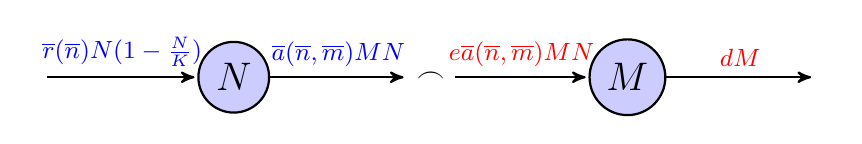
\begin{tikzpicture}[->,>=stealth',shorten >=1pt,auto,node distance=2.5cm, thick,main node/.style={circle,fill=blue!20,draw,font=\sffamily\Large\bfseries}]
	
			\node[main node] (1) {$N$};
			\node (midpt) [right of=1] {$\frown$};
			\node[main node] (2) [right of=midpt] {$M$};
			\node (input) [left of=1] {};
			\node (output) [right of=2] {};
	
			\path[every node/.style={font=\sffamily\small}]
			(input)	edge node {{\color{blue}$\overline{r}(\overline{n})N(1 - \frac{N}{K})$}} (1)
			(1)		edge node {{\color{blue}$\overline{a}(\overline{n}, \overline{m})MN$}} (midpt)
			(midpt)	edge node {{\color{red}$e\overline{a}(\overline{n}, \overline{m})MN$}} (2)
			(2)		edge node {{\color{red}$dM$}} (output);
		\end{tikzpicture}\vskip0.35cm
	\end{center}
	\vskip.25cm
	\begin{columns}
		\begin{column}{0.5\textwidth}
			{\bf Variables}
			\begin{itemize}
				\item \footnotesize{\color{blue}$N \equiv $ Prey Density}
				\item {\color{blue}$\overline{n} \equiv $ {\bf Average} Prey Trait Value}
				\item {\color{red}$M \equiv $ Predator Density}
				\item {\color{red}$\overline{m} \equiv $ {\bf Average} Predator Trait Value}
			\end{itemize}
		\end{column}
		\begin{column}{0.5\textwidth}
			{\bf Parameters}
			\begin{itemize}
				\item \footnotesize$\overline{r} \equiv $ Average Intrinsic Prey Growth \hphantom{$\overline{r} \equiv $} Rate Function
				\item $K \equiv $ Prey Carrying Capacity
				\item $d \equiv $ Predator Death Rate
				\item $e \equiv $ Efficiency
			\end{itemize}
		\end{column}
	\end{columns}
\end{frame}
\begin{frame}
	\frametitle{Evolutionary Components}
	\begin{itemize}
		\item The evolution of the average trait value is always \underline{in the direction} \underline{which increases the mean fitness in the population}. {\tiny[Lande, 1976]}
	\end{itemize}
	\begin{align*}
		\frac{d\overline{n}}{dt} &= \beta_G^2{\color{cyan}\frac{\partial \overline{Y}}{\partial \overline{n}}} = \beta_G^2{\color{cyan}\left[\overline{r}(\overline{n})\left(1 - \frac{N}{K}\right)\frac{(\phi - \overline{n})}{\beta^2 + \gamma^2} + \frac{M(\theta - (\overline{m} - \overline{n}))}{\sigma^2 + \beta^2 + \tau^2} \overline{a}(\overline{m}, \overline{n})\right]}\\[.1cm]
		\frac{d\overline{m}}{dt} &= \sigma_G^2{\color{magenta}\frac{\partial \overline{W}}{\partial \overline{m}}} = \sigma_G^2{\color{magenta}\frac{eN(\theta - (\overline{m} - \overline{n}))}{\sigma^2 + \beta^2 + \tau^2} \overline{a}(\overline{m}, \overline{n})}
	\end{align*}
	\vskip.25cm
	\begin{columns}
		\begin{column}{0.5\textwidth}
			{\bf Variables}
			\begin{itemize}
				\item \footnotesize$N \equiv $ Prey Density
				\item $\overline{n} \equiv $ {\bf Average} Prey Trait Value
				\item $M \equiv $ Predator Density
				\item $\overline{m} \equiv $ {\bf Average} Predator Trait Value
			\end{itemize}
		\end{column}
		\begin{column}{0.5\textwidth}
			{\bf Parameters}
			\begin{itemize}
				\item \footnotesize$\phi \equiv $ Prey Optimum Trait Value
				\item $\gamma^2 \equiv $ Stabilizing Selection Constant
				\item $\overline{r} \equiv $ Average Intrinsic Prey Growth \hphantom{$\overline{r} \equiv $} Rate Function
				\item \footnotesize$\beta_G^2 \equiv $ Prey genetic variance
				\item $\sigma_G^2 \equiv $ Predator genetic variance
			\end{itemize}
		\end{column}
	\end{columns}
\end{frame}
\begin{frame}
	\frametitle{The Complete $1\times1$ Model \\ (One Predator Species, One Prey Species)}
	{\bf Ecological Components}
	\begin{align*}
		\frac{dN}{dt} &= N\cdot {\color{blue}\overline{Y}(N, \overline{n}, M, \overline{m})}\ = N{\color{blue}\left[\overline{r}(\overline{n})\left(1 - \frac{N}{K}\right) - M\overline{a}(\overline{n}, \overline{m})\right]}\\[.1cm]
		\frac{dM}{dt} &= M\cdot {\color{red}\overline{W}(N, \overline{n}, M, \overline{m})} = M{\color{red}\left[eN\overline{a}(\overline{n}, \overline{m}) - d\right]}
	\end{align*}
	{\bf Evolutionary Components}
	\begin{align*}
		\frac{d\overline{n}}{dt} &= \beta_G^2{\color{cyan}\frac{\partial \overline{Y}}{\partial \overline{n}}} = \beta_G^2{\color{cyan}\left[\overline{r}(\overline{n})\left(1 - \frac{N}{K}\right)\frac{(\phi - \overline{n})}{\beta^2 + \gamma^2} + \frac{M(\theta - (\overline{m} - \overline{n}))}{\sigma^2 + \beta^2 + \tau^2} \overline{a}(\overline{m}, \overline{n})\right]}\\[.1cm]
		\frac{d\overline{m}}{dt} &= \sigma_G^2{\color{magenta}\frac{\partial \overline{W}}{\partial \overline{m}}} = \sigma_G^2{\color{magenta}\frac{eN(\theta - (\overline{m} - \overline{n}))}{\sigma^2 + \beta^2 + \tau^2} \overline{a}(\overline{m}, \overline{n})}
	\end{align*}
\end{frame}



% \begin{frame}
% 	\begin{center}
% 		\huge Ask us about our\\ preliminary $1 \times 2$ results!
% 	\end{center}
% \end{frame}




\section{Preliminary Results}
\subsection{$1 \times 1$}
\begin{frame}
	\frametitle{Equilibria - $1\times1$}
	\begin{align*}
		\begin{array}{ll}
			\dfrac{dN}{dt} = N\cdot {\color{blue}\overline{Y}(N, \overline{n}, M, \overline{m})} &\ \ \ \ \ \ \dfrac{d\overline{n}}{dt} = \beta_G^2{\color{cyan}\dfrac{\partial \overline{Y}}{\partial \overline{n}}} \\[.3cm]
			\dfrac{dM}{dt} = M\cdot {\color{red}\overline{W}(N, \overline{n}, M, \overline{m})} & \ \ \ \ \ \dfrac{d\overline{m}}{dt} = \sigma_G^2{\color{magenta}\dfrac{\partial \overline{W}}{\partial \overline{m}}}
		\end{array}
	\end{align*}
	{\bf Extinction} \uncover<2->{$\boxed{\text{\it Unstable}}$}
	\begin{align*}
		(N^*, M^*, \overline{n}^*, \overline{m}^*) = (0, 0, \underline{\ \ }, \underline{\ \ })
	\end{align*}
	{\bf Exclusion} \uncover<3->{$\boxed{\text{\it Locally stable under certain conditions}}$}
	\begin{align*}
		(N^*, M^*, \overline{n}^*, \overline{m}^*) = (K, 0, \underline{\ \ }, \underline{\ \ })
	\end{align*}
	\uncover<4->{{\bf Necessary Conditions for Locally Stable Exclusion:}}
	\begin{itemize}
		\item \uncover<4->{$d > e\overline{a}(\overline{m}^*, \overline{n}^*)K$}
		\item \uncover<4->{$((\overline{m}^* - \overline{n}^*) - \theta)^2 < \sigma^2 + \beta^2 + \tau^2$}
	\end{itemize}
\end{frame}
\begin{frame}
	\frametitle{Equilibria - $1\times1$}
	\begin{align*}
		\begin{array}{ll}
			\dfrac{dN}{dt} = N\cdot {\color{blue}\overline{Y}(N, \overline{n}, M, \overline{m})} &\ \ \ \ \ \ \dfrac{d\overline{n}}{dt} = \beta_G^2{\color{cyan}\dfrac{\partial \overline{Y}}{\partial \overline{n}}} \\[.3cm]
			\dfrac{dM}{dt} = M\cdot {\color{red}\overline{W}(N, \overline{n}, M, \overline{m})} & \ \ \ \ \ \dfrac{d\overline{m}}{dt} = \sigma_G^2{\color{magenta}\dfrac{\partial \overline{W}}{\partial \overline{m}}}
		\end{array}
	\end{align*}
	{\bf Coexistence} \uncover<2->{$\boxed{\text{\it Locally stable under certain conditions}}$}
	\begin{align*}
		(N^*, M^*, \overline{n}^*, \overline{m}^*) = (\dfrac{d\sqrt{A}}{e \alpha \tau}\ ,\ \dfrac{\rho\gamma\sqrt{A}}{\alpha\tau\sqrt{B}}\left(1 - \dfrac{d\sqrt{A}}{Ke\alpha\tau}\right)\ ,\ \theta\ ,\ \theta + \phi) \\[.1cm]
		\text{where $A = \sigma^2 + \beta^2 + \tau^2$ and $B = \beta^2 + \gamma^2$}
	\end{align*}
	\uncover<3->{{\bf Necessary Condition for Locally Stable Coexistence:}}
	\begin{itemize}
		\item \uncover<3->{$\dfrac{\sigma_G^2}{\beta_G^2} > \dfrac{\rho\gamma}{d\sqrt{B}}\left(1 - \dfrac{d\sqrt{A}}{Ke\alpha\tau}\right)\left(1 - \dfrac{A}{B}\right)$}
	\end{itemize}
\end{frame}

\begin{frame}
	\frametitle{Figures - $1\times1$ - Stable Exclusion}
	\begin{columns}[t]
		\begin{column}{.5\textwidth}
			\centering
			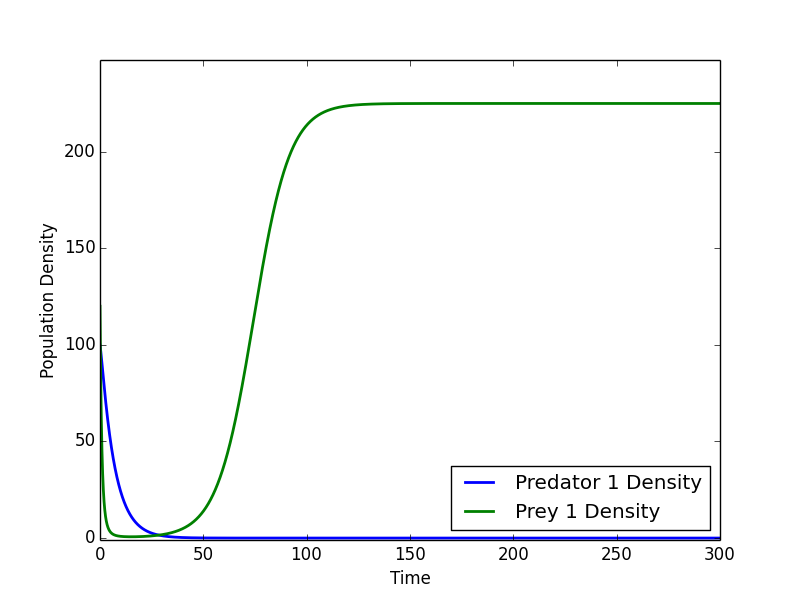
\includegraphics[width=5cm,height=3.75cm]{figures/1x1/variable_growth/stable_exclusion/densities.png}\\
			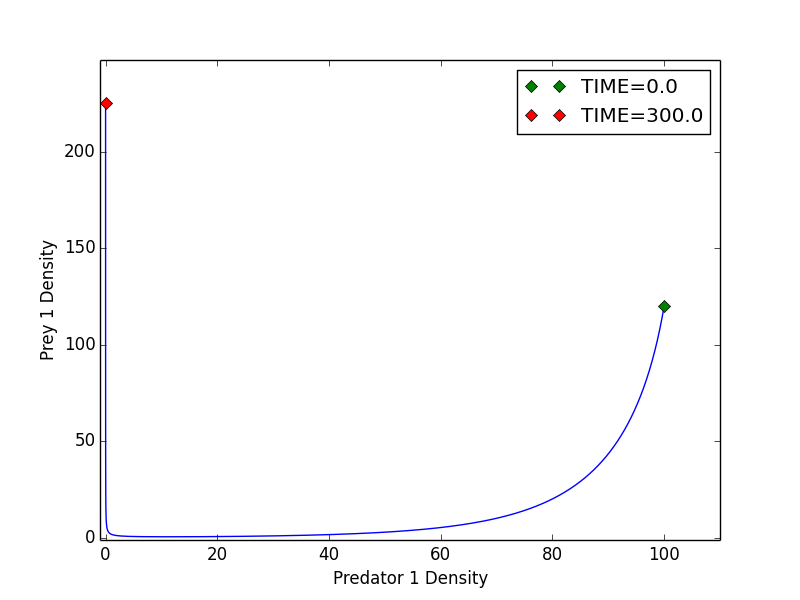
\includegraphics[width=5cm,height=3.75cm]{figures/1x1/variable_growth/stable_exclusion/density_phase_plane.png}
		\end{column}
		\begin{column}{.5\textwidth}
			\centering
			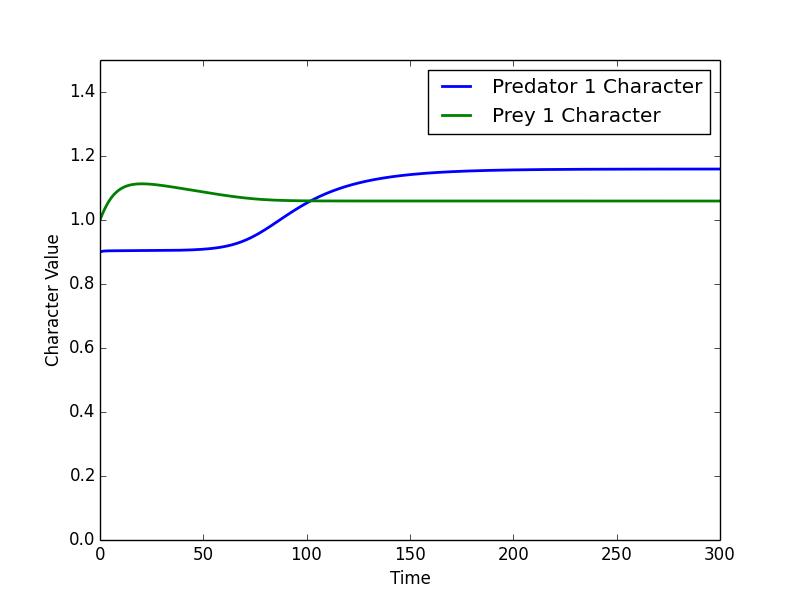
\includegraphics[width=5cm,height=3.75cm]{figures/1x1/variable_growth/stable_exclusion/traits.png}\\
			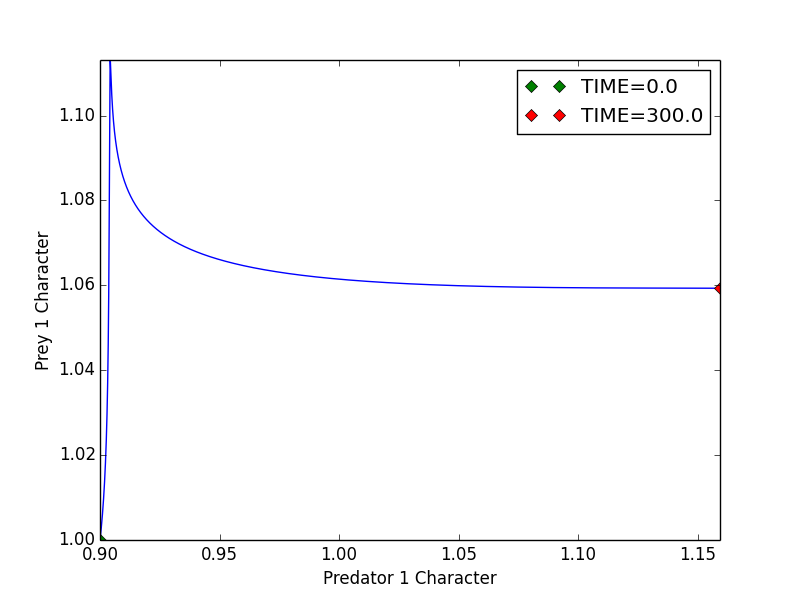
\includegraphics[width=5cm,height=3.75cm]{figures/1x1/variable_growth/stable_exclusion/trait_phase_plane.png}
		\end{column}
	\end{columns}
\end{frame}
\begin{frame}
	\frametitle{Figures - $1\times1$ - Stable Coexistence}
	\begin{columns}[t]
		\begin{column}{.5\textwidth}
			\centering
			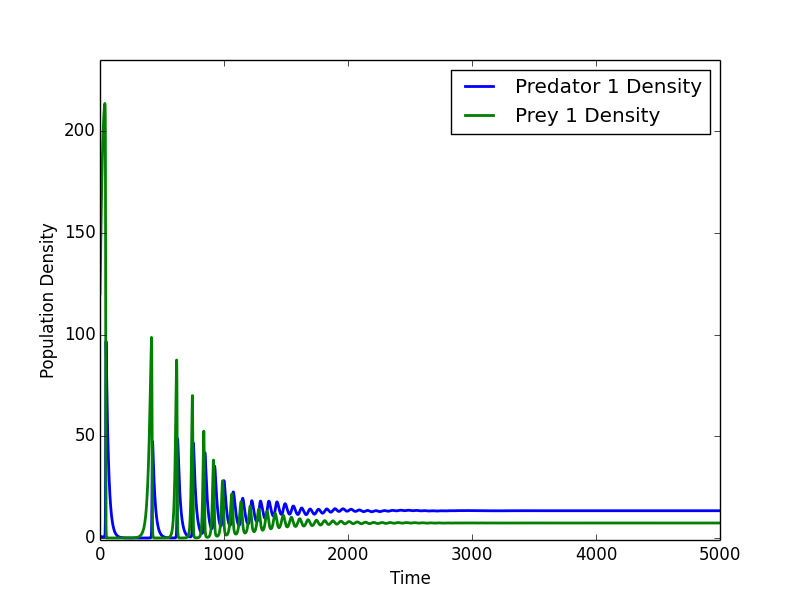
\includegraphics[width=5cm,height=3.75cm]{figures/1x1/variable_growth/stable_coexistence/densities.png}\\
			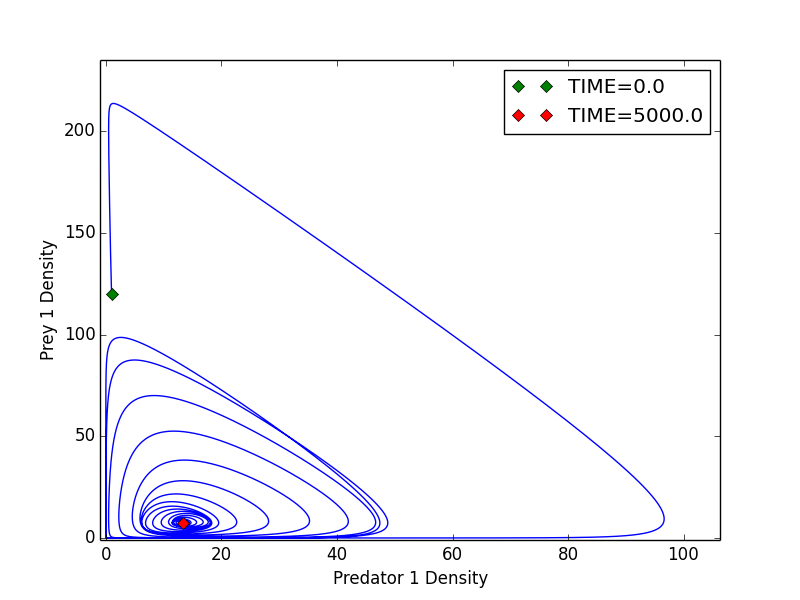
\includegraphics[width=5cm,height=3.75cm]{figures/1x1/variable_growth/stable_coexistence/density_phase_plane.png}
		\end{column}
		\begin{column}{.5\textwidth}
			\centering
			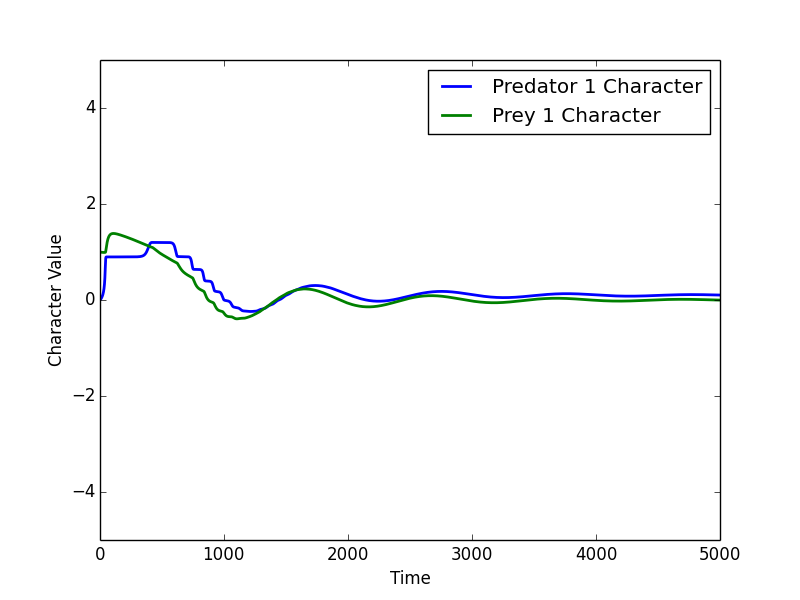
\includegraphics[width=5cm,height=3.75cm]{figures/1x1/variable_growth/stable_coexistence/traits.png}\\
			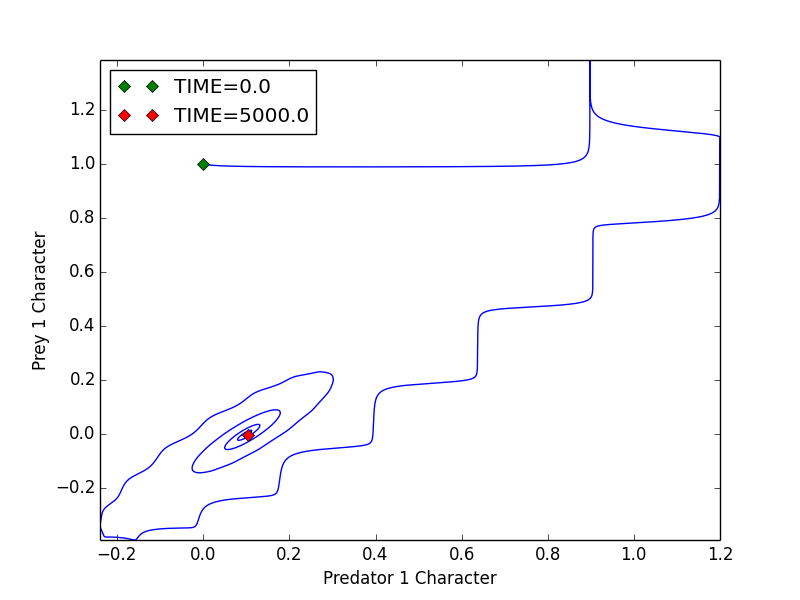
\includegraphics[width=5cm,height=3.75cm]{figures/1x1/variable_growth/stable_coexistence/trait_phase_plane.png}
		\end{column}
	\end{columns}
\end{frame}
\begin{frame}
	\frametitle{Figures - $1\times1$ - Stable Cycles {\normalsize(Red Queen Dynamics)}{\tiny[Kindrik, Kondrashov, 1994]}}
	\begin{columns}[t]
		\begin{column}{.5\textwidth}
			\centering
			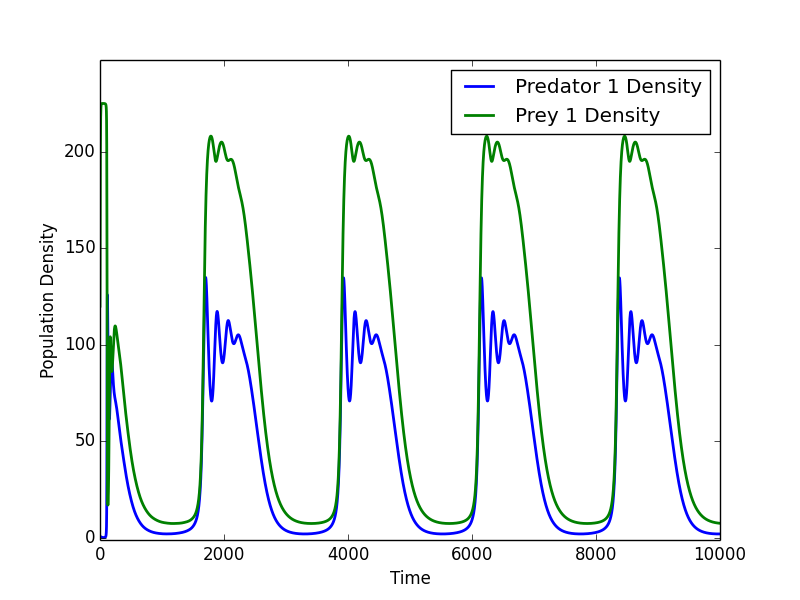
\includegraphics[width=5cm,height=3.75cm]{figures/1x1/variable_growth/stable_cycles/densities.png}\\
			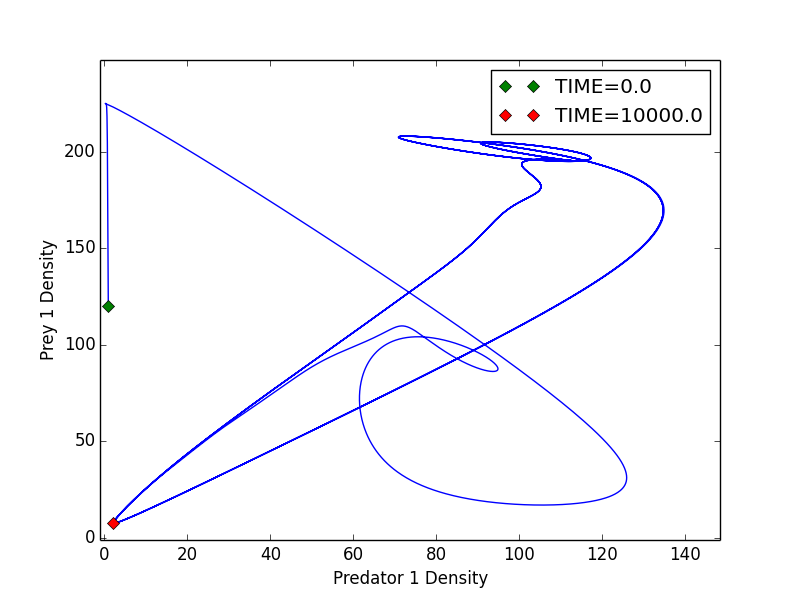
\includegraphics[width=5cm,height=3.75cm]{figures/1x1/variable_growth/stable_cycles/density_phase_plane.png}
		\end{column}
		\begin{column}{.5\textwidth}
			\centering
			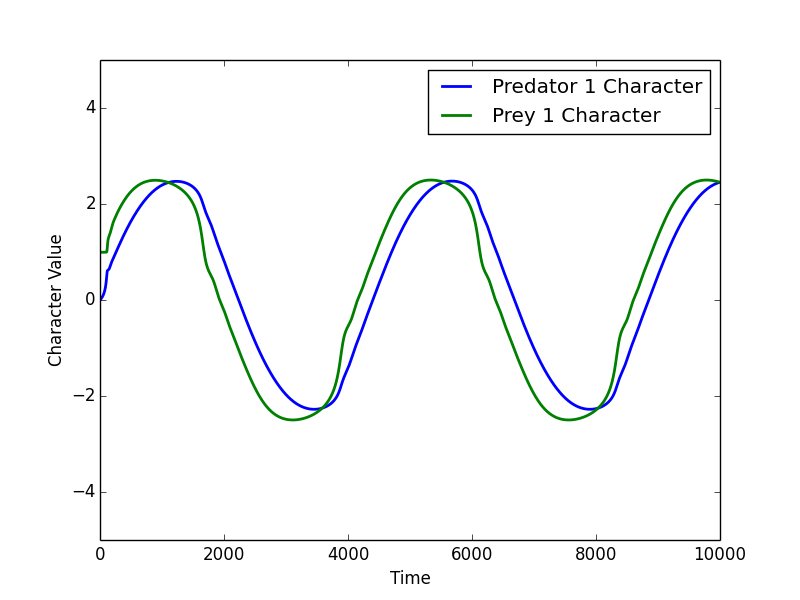
\includegraphics[width=5cm,height=3.75cm]{figures/1x1/variable_growth/stable_cycles/traits.png}\\
			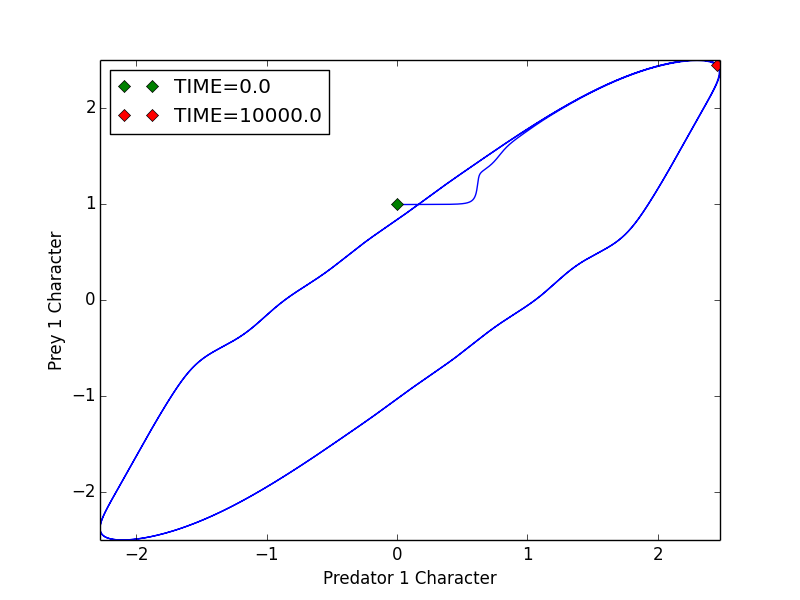
\includegraphics[width=5cm,height=3.75cm]{figures/1x1/variable_growth/stable_cycles/trait_phase_plane.png}
		\end{column}
	\end{columns}
\end{frame}

\subsection*{General Ditrophic Expansion}
\begin{frame}
	\frametitle{Expansion of Fitness Functions}
	{\bf Prey Fitness}
	\begin{align*}
		{\color{blue}Y(N, n, M, m)} &= r(n)\left(1 - \frac{N}{K}\right) - Ma(n, m) \\
		\uncover<2->{\scriptsize&\downarrow} \\
		\uncover<2->{{\color{blue}Y_j(N_j, n_j, [M_i]_{i=1}^{u}, [m_i]_{i=1}^{u})} &= r_j(n_j)\left(1 - \frac{N_j}{K_j}\right) - \sum\limits_{i = 1}^{u}M_ia_{ij}(n_j, m_i)}
	\end{align*}
	{\bf Predator Fitness}
	\begin{align*}
		{\color{red}W(N, n, M, m)} &= eNa(n, m) - d \\
		\uncover<3->{\scriptsize&\downarrow} \\
		\uncover<3->{{\color{red}W_i([N_j]_{j=1}^{v}, [n_j]_{j=1}^{v}, M_i, m_i)} &= \sum\limits_{j = 1}^{v}\Big[e_{ij}N_ja_{ij}(n_j, m_i)\Big] - d_i}
	\end{align*}
	\uncover<2->{\begin{center}{\bf Notation:} $[x_i]_{i=1}^{u} = x_1, \dots, x_u$\end{center}}
\end{frame}
\begin{frame}
	\frametitle{Average Fitness Calculation}
	\begin{align*}
		{\color{blue}\overline{Y}_j(N_j, \overline{n_j}, [M_i]_{i=1}^{u}, }&{\color{blue}[\overline{m_i}]_{i=1}^{u})} \\
		&= \int\limits_{\mathbb{R}^{u+1}} Y_j \cdot \prod\limits_{i=1}^{u}\Big[p_i(m_i, \overline{m_i})\Big] \cdot p(n, \overline{n}) \prod\limits_{i=1}^{u}\Big[dm_i\Big] dn_j\\
		&= {\color{blue}\overline{r_j}(\overline{n_j})\left(1 - \frac{N_j}{K_j}\right) - \sum\limits_{i = 1}^{u}M_i\overline{a}_{ij}(\overline{n}_j, \overline{m}_i)}
	\end{align*}
	\begin{align*}
		{\color{red}\overline{W}_i(N_j, \overline{n_j}, [M_i]_{i=1}^{u}, }&{\color{red}[\overline{m_i}]_{i=1}^{u})} \\
		&= \int\limits_{\mathbb{R}^{u+1}} W_i \cdot p_i(m_i, \overline{m_i}) \cdot \prod\limits_{j=1}^{v}\Big[p(n_j, \overline{n}_j)\Big] dm_i \prod\limits_{j=1}^{v}\Big[dn_j\Big]\\
		&= {\color{red}\sum\limits_{j = 1}^{v}\Big[e_{ij}N_j\overline{a}_{ij}(\overline{n}_j, \overline{m}_i)\Big] - d_i}
	\end{align*}
\end{frame}
\begin{frame}
	\frametitle{The Complete $u\times v$ Model - \normalsize($u$ Predator Species, $v$ Prey Species)}
	{\bf Ecological Components}
	\begin{align*}
		\frac{dN_j}{dt} &= N_j{\color{blue}\overline{Y_j}} = N_j {\color{blue}\left[{\color{blue}\overline{r_j}(\overline{n_j})\left(1 - \frac{N_j}{K_j}\right) - \sum\limits_{i = 1}^{u}M_i\overline{a}_{ij}(\overline{n}_j, \overline{m}_i)}\right]} \\
		\frac{dM_i}{dt} &= M_i{\color{red}\overline{W_i}} = M_i {\color{red}\left[\sum\limits_{j = 1}^{v}\Big[e_{ij}N_j\overline{a}_{ij}(\overline{m}_i, \overline{n}_j)\Big] - d_i\right]}
	\end{align*}
	{\bf Evolutionary Components}
	\begin{align*}
		\frac{d\overline{n}_j}{dt} &= \beta_{Gj}^2{\color{cyan}\frac{\partial \overline{Y_j}}{\partial \overline{n_j}}} = \beta_{Gj}^2{\color{cyan}\left[\overline{r_j}(\overline{n_j})\left(1 - \frac{N_j}{K_j}\right)\frac{(\phi_j - \overline{n_j})}{\beta_j^2 + \gamma_j^2}\right.}
		\\&\hphantom{\text{mmmmmmmmmmm}}{\left.\color{cyan}+ \sum\limits_{i=1}^{u}\left[\frac{M_i(\theta_{ij} - (\overline{m_i} - \overline{n_j}))}{\sigma_i^2 + \beta_j^2 + \tau_{ij}^2} \overline{a}_{ij}(\overline{m_i}, \overline{n_j})\right]\right]}\\
		\frac{d\overline{m}_i}{dt} &= \sigma_{Gi}^2{\color{magenta}\sum\limits_{j=1}^{v}\left[\frac{e_{ij}N_j(\theta_{ij} - (\overline{m_i} - \overline{n_j}))}{\sigma_i^2 + \beta_j^2 + \tau_{ij}^2} \overline{a}_{ij}(\overline{m_i}, \overline{n_j})\right]}
	\end{align*}
\end{frame}
\begin{frame}
	\frametitle{The Complete $u\times v$ Model - \normalsize($u$ Predator Species, $v$ Prey Species)}
	\Wider[6em]{
	\begin{center}
		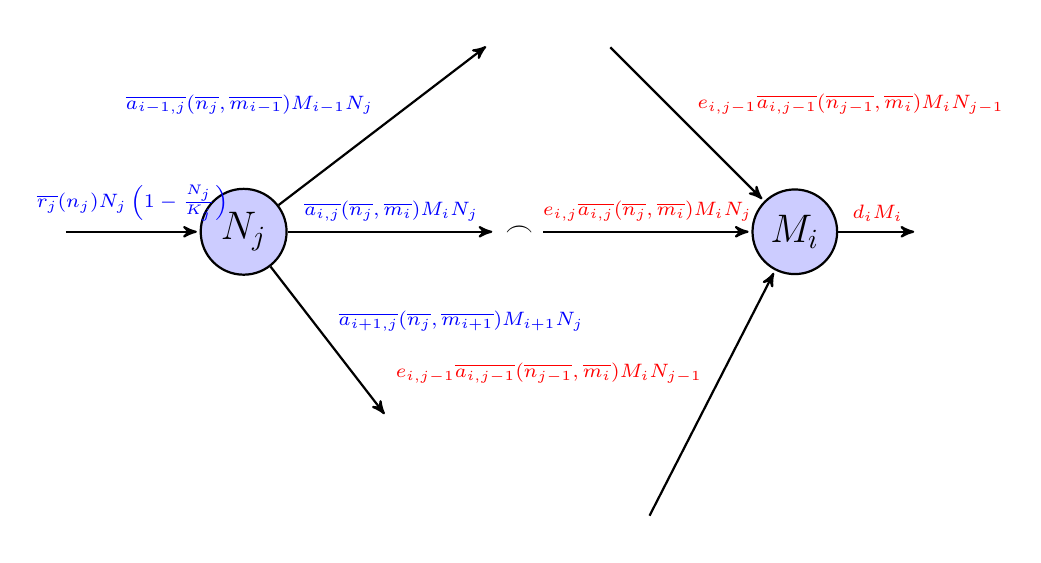
\begin{tikzpicture}[->,>=stealth',shorten >=1pt,auto,node distance=3.5cm, thick,main node/.style={circle,fill=blue!20,draw,font=\sffamily\Large\bfseries}]
	
			\node[main node] (n1) {$N_j$};
			\node (midpt1) [right of=n1] {$\frown$};
			\node[main node] (m1) [right of=midpt1] {$M_i$};
			\node (input1) [left =1.7cm of n1] {};
			\node (output1) [right = 1cm of m1] {};
			\node (upright) [above right of=n1] {};
			\node (furtherright) [right = .5cm of upright] {};
			\node (downright) [below right of=n1] {};
			\node (alittleleft) [left = 0.3cm of downright] {};
			\node (upleft) [above left of=m1] {};
			\node (downleft) [below left of=m1] {};
			\node (furtherdown) [below = 1cm of downleft] {};
			\node (alittleright) [right = 0.3cm of furtherdown] {};
	
			\path[every node/.style={font=\sffamily\small}]
			(input1)	edge node {\scriptsize{\color{blue}$\overline{r_j}(n_j)N_j\left(1 - \frac{N_j}{K_j}\right)$}} (n1)
			(n1)		edge node {\scriptsize{\color{blue}$\overline{a_{i,j}}(\overline{n_j}, \overline{m_i})M_iN_j$}} (midpt1)
					edge node {\scriptsize{\color{blue}$\overline{a_{i-1,j}}(\overline{n_j}, \overline{m_{i-1}})M_{i-1}N_j$}} (furtherright)
					edge node {\scriptsize{\color{blue}$\overline{a_{i+1,j}}(\overline{n_j}, \overline{m_{i+1}})M_{i+1}N_j$}} (alittleleft)
			(midpt1)	edge node {\scriptsize{\color{red}$e_{i,j}\overline{a_{i,j}}(\overline{n_j}, \overline{m_i})M_iN_j$}} (m1)
			(m1)		edge node {\scriptsize{\color{red}$d_iM_i$}} (output1)
			(upleft)	edge node {\scriptsize{\color{red}$e_{i,j-1}\overline{a_{i,j-1}}(\overline{n_{j-1}}, \overline{m_i})M_iN_{j-1}$}} (m1)
			(alittleright)	edge node {\scriptsize{\color{red}$e_{i,j-1}\overline{a_{i,j-1}}(\overline{n_{j-1}}, \overline{m_i})M_iN_{j-1}$}} (m1)
			;
		\end{tikzpicture}\vskip0.35cm
	\end{center}
	}
\end{frame}

\section{Future Work}
\begin{frame}
	\frametitle{Future Work}
	\begin{itemize}
		\item Two prey species in apparent competition via one generalist predator
		\item Two predator species in competition for one prey
		\item One specialist predator competing with one generalist predator for two prey
		\item Two specialist predators competing with one generalist predator for two prey species
		\item Further analysis of the general $u \times v$ model
		\item Intraguild predation
	\end{itemize}
\end{frame}

\begin{frame}
	\frametitle{Thank You!}
	\begin{itemize}
		\item PUMP (Preparing Undergraduates through Mentoring towards PhDs)
		\item Pacific Math Alliance
		\item National Math Alliance
		\item Dr. Helena Noronha, Dr. Ramin Vakilian, and all other PUMP organizers
		\item National Science Foundation
		\item California State University, Northridge
		\item Dr. Jing Li and Dr. Casey terHorst
	\end{itemize}
	\begin{center}
		{\Huge Questions?}
	\end{center}
\end{frame}

% \begin{frame}
% 	\frametitle{Equilibria - $1\times2$}
% 	\begin{align*}
% 		\begin{array}{ll}
% 			\dfrac{dN_1}{dt} = N_1\cdot \overline{Y}_1(\overline{m}, \overline{n}_1, M, N_1) &\ \ \ \ \ \ \dfrac{d\overline{n}_1}{dt} = \beta_{G1}^2\dfrac{\partial \overline{Y}_1}{\partial \overline{n}_1} \\[.3cm]
% 			\dfrac{dN_2}{dt} = N_2\cdot \overline{Y}_2(\overline{m}, \overline{n}_2, M, N_2) &\ \ \ \ \ \ \dfrac{d\overline{n}_2}{dt} = \beta_{G2}^2\dfrac{\partial \overline{Y}_2}{\partial \overline{n}_2} \\[.3cm]
% 			\dfrac{dM}{dt} = M\cdot \overline{W}(\overline{m}, \overline{n}_1, \overline{n}_2, N_1, N_2) & \ \ \ \ \ \ \dfrac{d\overline{m}}{dt} = \sigma_G^2\dfrac{\partial \overline{W}}{\partial \overline{m}}
% 		\end{array}
% 	\end{align*}
% 	\uncover<2->{{\bf Extinction}} \uncover<3->{$\boxed{\text{\it Unstable}}$}
% 	\begin{align*}
% 		\uncover<2->{(N_1^*, N_2^*, M^*, \overline{n}_1^*, \overline{n}_2^*, \overline{m}^*) = (0, 0, 0, \underline{\ \ }, \underline{\ \ }, \underline{\ \ })}
% 	\end{align*}
% 	\uncover<4->{{\bf Exclusion}} \uncover<5->{$\boxed{\text{\it Stable under certain conditions}}$}
% 	\begin{align*}
% 		\uncover<4->{(N_1^*, N_2^*, M^*, \overline{n}_1^*, \overline{n}_2^*, \overline{m}^*) &= (K_1, K_2, 0, \underline{\ \ }, \underline{\ \ }, \underline{\ \ })}
% 	\end{align*}
% \end{frame}
% \begin{frame}
% 	\frametitle{Equilibria - $1\times2$}
% 	\begin{align*}
% 		\begin{array}{ll}
% 			\dfrac{dN_1}{dt} = N_1\cdot \overline{Y}_1(\overline{m}, \overline{n}_1, M, N_1) &\ \ \ \ \ \ \dfrac{d\overline{n}_1}{dt} = \beta_{G1}^2\dfrac{\partial \overline{Y}_1}{\partial \overline{n}_1} \\[.3cm]
% 			\dfrac{dN_2}{dt} = N_2\cdot \overline{Y}_2(\overline{m}, \overline{n}_2, M, N_2) &\ \ \ \ \ \ \dfrac{d\overline{n}_2}{dt} = \beta_{G2}^2\dfrac{\partial \overline{Y}_2}{\partial \overline{n}_2} \\[.3cm]
% 			\dfrac{dM}{dt} = M\cdot \overline{W}(\overline{m}, \overline{n}_1, \overline{n}_2, N_1, N_2) & \ \ \ \ \ \ \dfrac{d\overline{m}}{dt} = \sigma_G^2\dfrac{\partial \overline{W}}{\partial \overline{m}}
% 		\end{array}
% 	\end{align*}
% 	\uncover<2->{{\bf Generalist Becomes Specialist}} \uncover<3->{$\boxed{\text{\it Stable under certain conditions???}}$}
% 	\begin{align*}
% 		\uncover<2->{&(N_1^*,N_2^*,M^*,\overline{n}_1^*,\overline{n}_2^*,\overline{m}^*) \\[.1cm]
% 		=\ &(\dfrac{d\sqrt{A_1}}{e_1 \alpha_1 \tau_1}\ ,\ K_2\ ,\ \dfrac{r_1\sqrt{A_1}}{\alpha_1\tau_1}\left(1 - \dfrac{d\sqrt{A_1}}{K_1e_1\alpha_1\tau_1}\right)\ ,\ \mu_1^*\ ,\ \mu_2^*\ ,\ \mu_1^* - \theta_1)}
% 	\end{align*}
% 	\uncover<2->{where $A_1 = \sigma^2 + \beta_1^2 + \tau_1^2$, $\mu_1^*$ is an arbitrary value, and $\mu_2^*$ is sufficiently far from $\mu_1^* - \theta_1$.}

% \end{frame}

% \begin{frame}
% 	\frametitle{Figures - $1\times2$}
% 	{\bf Generalist Becomes Specialist}
% 	\Wider[6em]{
% 	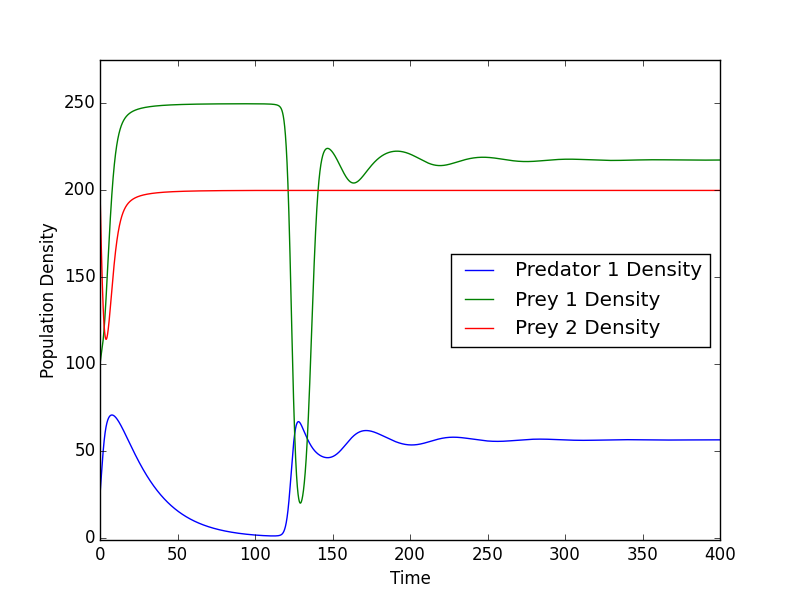
\includegraphics[scale=0.3175]{figures/1x2/densities_generalist_to_specialist.png}
%    	\hfill
%    	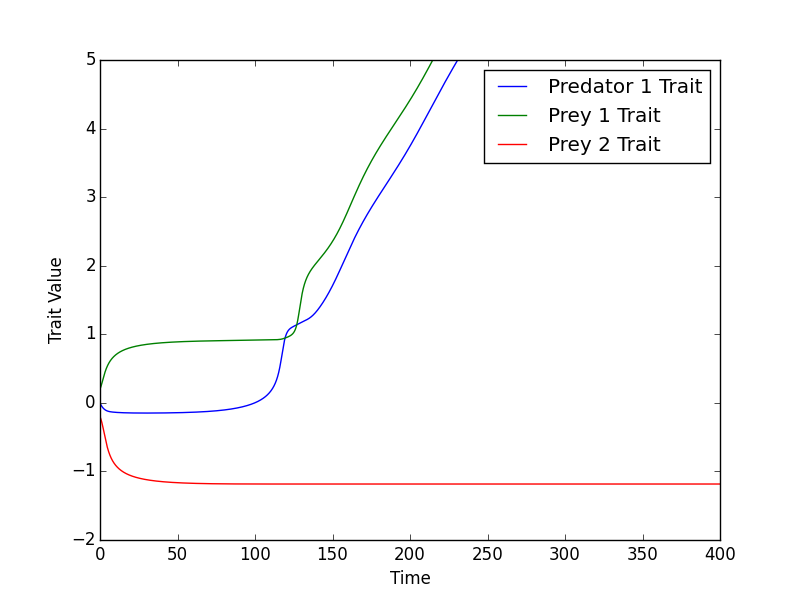
\includegraphics[scale=0.3175]{figures/1x2/traits_generalist_to_specialist.png}
% 	}
% \end{frame}
% \begin{frame}
% 	\frametitle{Figures - $1\times2$}
% 	{\bf Unstable Coexistence}
% 	\Wider[6em]{
% 	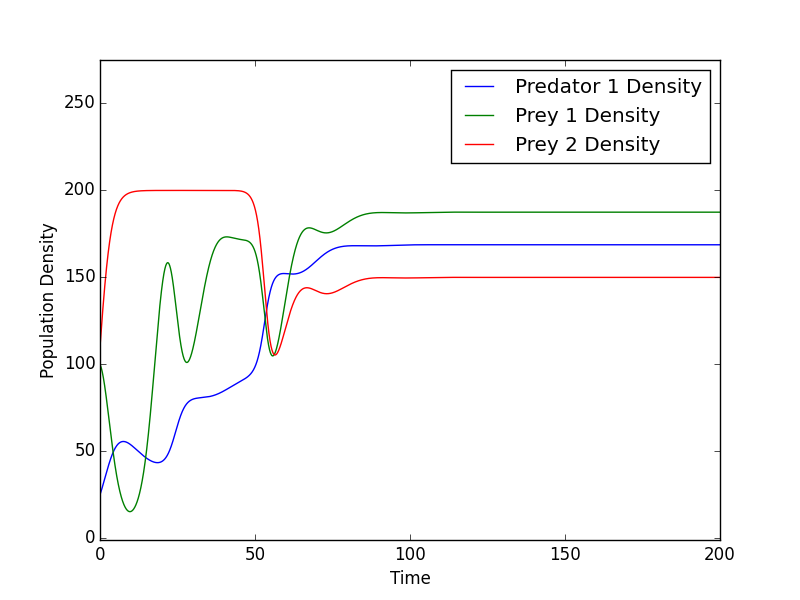
\includegraphics[scale=0.3175]{figures/1x2/densities_unstable_coexistence.png}
%    	\hfill
%    	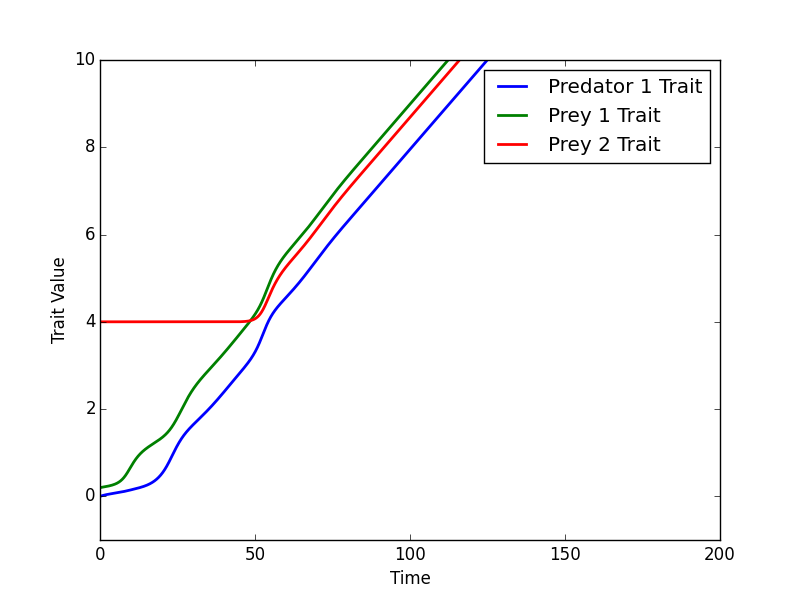
\includegraphics[scale=0.3175]{figures/1x2/traits_unstable_coexistence.png}
% 	}
% \end{frame}





\end{document}